\documentclass[submission,copyright,creativecommons]{../lib/eptcs}
\providecommand{\event}{ECAL 2013} % Name of the event you are submitting to

\usepackage[utf8]{inputenc}
\usepackage{lmodern}
\usepackage[T1]{fontenc}
\usepackage{amsfonts}
\usepackage{amssymb}

\usepackage{slovak}
\usepackage{fontenc}
\usepackage{graphicx}
\usepackage{graphics}
\usepackage{graphicx}
\usepackage{hyperref}
\usepackage{makeidx}

\newtheorem{definition}{Definition}[section]
\newtheorem{HLPpoznamka}{Note}[section]
\newtheorem{HLPpriklad}{Example}[section]
\newtheorem{HLPcvicenie}[HLPpriklad]{Exercise}
\newtheorem{HLPdokaz}{Proof}[section]
\newtheorem{zadanie}{Task}[section]
\newenvironment{poznamka}{\begin{HLPpoznamka}\rm}{\end{HLPpoznamka}}
\newenvironment{example}{\begin{HLPpriklad}\rm}{\end{HLPpriklad}}
\newenvironment{cvicenie}{\begin{HLPcvicenie}\rm}{\end{HLPcvicenie}}
\newenvironment{dokaz}{\begin{HLPdokaz}\rm}{\end{HLPdokaz}}
\newtheorem{veta}{Theorem}[section]
\newtheorem{lemma}[veta]{Lemma}
\newtheorem{dosledok}[veta]{Corollary}
\newtheorem{teza}[veta]{Proposition}


\pagestyle{headings}
\bibliographystyle{../lib/eptcs}

\def\eps{\varepsilon}
\def\goodgap{\hspace{\subfigcapskip}}
\renewcommand\refname{References}

% Itemize bulet types
\renewcommand{\labelitemi}{$\bullet$}
\renewcommand{\labelitemii}{$\cdot$}

\begin{document}
\title{Inhibiting the parallelism in P systems}
\def\titlerunning{Inhibiting the parallelism in P systems}
\author{Michal Kováč}
\def\authorrunning{Michal Kováč}
\date{\today}
\maketitle

\begin{abstract}
P systems are formal models of distributed parallel multiset processing. Many variants make use of the maximal parallelism to achieve universality.
It is known that P systems with catalytic rules with only one catalyst are not universal, but when using promoters and inhibitors, the universality is achieved.
The sequential variant of P system is also not universal and we will show how the computational universality can be reached by using sequential P systems with inhibitors. Both accepting and generating case are investigated.
In addition, a new variant of P system is defined in this paper, where the emptiness of a region is represented by a special vacuum object. This variant is shown to be universal when operating in the sequential mode.
\end{abstract}

\section{Introduction}
\label{sec:introduction}

% Bio motivation

Membrane systems (P systems) were introduced by P\u{a}un (see \cite{Paun2000108}) as distributed parallel computing devices inspired by the structure and functionality of cells.
One of the objectives is to relax the condition of using the rules in a maximally parallel way in order to find more realistic P systems from a biological point of view.
In sequential systems, only one rewriting rule is used in each step of computation.

% Our work

We are looking for ways to obtain universality in this sequential mode.

% Inhibitors

At first, we consider inhibitors and show that using them we can simulate P system working in a maximally parallel way.

% Vacuum

Then, we introduce the concept of vacuum. In the common sense, vacuum represents a state of space with no or a little matter in it. Using vacuum in modelling frameworks can help express certain phenomena more easily.
We define a new P system variant, which creates a special vacuum object in a region as soon as the region becomes empty. The vacuum is removed whenever some object interacts with it. After the interaction, there is vacuum no longer. This removal process is realized by allowing the vacuum object to be used only on the left side of rules.
If we made the vacuum to be removed automatically when an object enters the region, there would be no difference with the variant without vacuum objects because of no interactions with it.
We are interested in how the variant with the vacuum improves the computational power of a P system in comparison to the variant without the vacuum.


% Related work

There have been lot of research that consider rewriting rules with catalysts, promoters and inhibitors. However, they were only used to overcome the limitations brought by non-cooperative rules, and still working in a maximal parallel manner.

% Max 1 instance of any rule

In \cite{Ibarra04dang} they have a variant of P systems with maximal parallelism restricted to use at most one instance of any rule in a step.
They show that for universality is sufficient non-cooperative variant where the only allowed cooperative rule with both symbols equal. For example rule $a|a\rightarrow b$. Also, catalytic rules are sufficient too.

% Cooperative vs Context free

In \cite{Sburlan05dragos} the author formally proves equality between classes of P systems and Parikh images of classes in Chomsky hierarchy. P systems with context-free rules are equal to $PsCF$ and P systems with cooperative rules are universal (equal to $PsRE$).

% Two catalysts are enough
% One catalyst with promoters / inhibitors is enough

The gap between is filled in \cite{Ionescu:jucs_10_5:on_p_systems_with}. Assumed P systems with context-free rules and maximal parallelism, there is a need for some context added to the rules. Cooperative or catalytic rules are sufficient for universality. The paper shows that two catalyst are enough. There was an open question whether one catalyst is enough. Then it was shown that it is not enough unless we allow promoters or inhibitors. Without them it has the power of Lindenmayer systems.

% Inhibiting rules

Rewriting controlled by inhibition is more thoroughly researched in \cite{Cavaliere:2004:IRP:2144633.2144648}. P systems with context-free rules and are enriched with rules with option to inhibit / de-inhibit another rule. This, with one catalyst is shown to be universal. Without catalyst and with only one membrane it is shown to have at least the power of Lindenmayer systems.

% Context free with inhibitors

However, \cite{doi:10.1142/S0129054106003772} shows that even if we have maximal parallel context-free rules with inhibitors, it is only equal to the family of Parikh sets of ET0L languages (PsET0L). If we have promoters instead of inhibitors, only the inclusion of the family PsET0L was proved. % it is stronger than PsET0L

% Sequential with energies and priorities

Several sequential variants of P systems were studied. In \cite{Freund:2004:SPS:2149813.2149831} membranes have been assigned energy values that can control rule rewriting. Each rule has energy that is consumed when the rule is applied. If we have rules with priorities, the system becomes universal.

% Sequential not universal

However, if we extend sequential P systems with cooperative rules as in \cite{Dang04onp} and restrict it to use only one membrane, it defines exactly semilinear sets and is not universal.

There is something fundamental that prevents the sequential systems to be universal. Unlike maximal parallel systems, the application of rules in sequential systems are not synchronized between membranes. Even inside one membrane an object can be rewritten multiple times while other objects are not rewritten at all.
Maximal parallelism does not suffer from these issues.

There is also a notion of minimal parallelism (\cite{Ciobanu:2007:PSM:1243519.1243811}), which forces all membranes to apply at least one rule if there is one that can be used. This approach solves the synchronization issue between membranes, but not the one inside one membrane. Nevertheless, P systems with minimal parallelism are universal.



% Deterministic, asynchronous context-free with inhibitors not universal

In \cite{Alhazov13} several non-cooperative variants with either promoters or inhibitors were studied. Maximally parallel and asynchronous modes was shown to be universal. They also defined the deterministic mode (only for accepting case). The computation is accepted only if for each configuration there was at most one multiset of rules applicable. Such deterministic variant was shown to only accept the family of all finite languages.

% CLS

Another sequential model, but not a variant of P system, is Calculi of Looping Sequences. It is introduced in \cite{Barbuti07thecalculus} as a membrane model where objects are strings that can loop around forming a membrane. Rewriting rules are global and are executed sequentially. It is shown to be universal by directly simulating P systems.


In section~\ref{sec:preliminaries} we recall some fundamental notions which we will use through the rest of the paper.
We introduce the notion of P system and define a computation of a P system in section~\ref{sec:p-systems}.
Some existing P system variants are mentioned in section~\ref{sec:variants}. There is also introduced our new variant of P system with vacuum.
In section~\ref{sec:inhibitors} we make a proof that sequential P systems with inhibitors are universal.
Similar result, but for our new variant of P system with vacuum is achieved and proven in section~\ref{sec:vacuum}.

\section{Preliminaries}
\label{sec:preliminaries}

Here we recall several notions from the classical theory of formal languages.

An {\bf alphabet} is a finite nonempty set of symbols. Usually it is denoted by $\Sigma$ or $V$. A {\bf string} over an alphabet is a finite sequence of symbols from alphabet. We denote by $V^*$ the set of all strings over an alphabet $V$. By $V^+$ = $V^* - \{\eps\}$ we denote the set of all nonempty strings over V. A {\bf language} over the alphabet $V$ is any subset of $V^*$.

The number of occurrences of a given symbol $a\in V$ in the string $w\in V^*$ is denoted by $|w|_a$. $\Psi_V(w)=(|w|_{a_1},|w|_{a_2},\dots,|w|_{a_n})$ is called a Parikh vector associated with the string $w\in V^*$, where $V=\{a_1,a_2,\dots a_n\}$. For a language $L\subseteq V^*$, $\Psi_V(L)=\{\Psi_V(w)|w\in L\}$ is the Parikh mapping associated with $V$. If FL is a family of languages, by PsFL is denoted the family of Parikh images of languages in FL.

A multiset over a set $X$ is a mapping $M: X\rightarrow \mathbb N$.
We denote by $M(x), x\in X$ the multiplicity of $x$ in the multiset $M$.
The {\bf support} of a multiset $M$ is the set $supp(M)=\{x\in X|M(x)\geq 1\}$.
It is the set of items with at least one occurrence.
A multiset is {\bf empty} when its support is empty.
A multiset $M$ with finite support $X = \{x_1, x_2, \dots, x_n\}$ can be represented by the string $x_1^{M(x_1)}x_2^{M(x_2)}\dots x_n^{M(x_n)}$.
As elements of a multiset can also be strings, we separate them with the pipe symbol, e.g. $element|element|other\_element$.
We say that multiset $M_1$ is included in multiset $M_2$ if $\forall x \in X: M_1(x)\leq M_2(x)$.
We denote it by $M_1\subseteq M_2$.
The {\bf union} of two multisets $M_1\cup M_2$ is a multiset where $\forall x \in X: (M_1\cup M_2)(x)=M_1(x)+M_2(x)$.
The {\bf difference} of two multisets $M_1-M_2$ is a multiset where $\forall x \in X: (M_1-M_2)(x)=M_1(x)-M_2(x)$.
Product of multiset $M$ with natural number $n\in \mathbb N$ is a multiset where $\forall x \in X: (n\cdot M)(x)=n\cdot M(x)$.
  
\section{P-systems}
\label{sec:p-systems}

%TODO: definovat simulaciu, ...

% Membrane structure

The fundamental ingredient of a P system is the {\bf membrane structure} (see \cite{Paun2006Introduction}). It is a hierarchically arranged set of membranes, all contained in the {\bf skin membrane}. A membrane without any other membrane inside is said to be {\bf elementary}. Each membrane determines a compartment, also called region, the space delimited from above by it and from below by the membranes placed directly inside, if any exists. Clearly, the correspondence membrane – region is one-to-one, that is why we sometimes use interchangeably these terms.

% Maximal parallelism

Consider a finite set of symbols $V=\{a_1, a_2,\dots, a_n\}$. An arbitrary multiset rewriting rule is a pair $(u, v)$ of multisets over the set $V$ where $u$ is not empty. Such a rule is typically written as $u\rightarrow v$. For a multiset rewriting rule $r : u\rightarrow v$, let $left(r) = u$ and $right(r) = v$. Let $w$ be a multiset of symbols over $V$ and let $R=\{r_1, r_2,\dots, r_k\}$ be a set of multiset rewriting rules such that $r_i = u_i\rightarrow v_i$ with $u_i, v_i$ multisets over $V$. Denote by $R^{ap}_w\subseteq R$ the {\bf set of applicable multiset rewriting rules} to $w$, that is, $R^{ap}_w = \{r\in R|left(r)\subseteq w\}$. Denote by $R^{msap}_w: R\rightarrow \mathbb N$, a multiset over $R$ of {\bf maximal simultaneously applicable multiset rewriting rules} to $w$. $R^{msap}_w$ is any multiset such that $\displaystyle\bigcup_{r\in R} R^{msap}_w(r)\cdot left(r)\subseteq w$ and $\forall r' \left(\displaystyle\bigcup_{r\in R} R^{msap}_w(r)\cdot left(r)\right)\cup left(r')\nsubseteq w$. In other words, we use a multiset of rewriting rules such that no more rules can be applied simultaneously.

% P system

Let $\Sigma$ be a set of objects. Recall that $\mathbb N^\Sigma$ contains all multisets of objects from $\Sigma$. {\bf Membrane configuration} is a tuple $(T, l, c)$, where:
\begin{itemize}
  \item $T$ is a rooted tree,
  \item $l\in\mathbb N^{V(T)}$ is a mapping that assigns for each node of $T$ a number (label), where $l(r_T)=1$, so the skin membrane is always labeled with 1,
  \item $c\in(\mathbb N^\Sigma)^{V(T)}$ is a mapping that assigns for each node of $T$ a multiset of objects from $\Sigma$, so it represents the contents of the membrane.
\end{itemize}

{\bf Active P system} is a tuple $(\Sigma, C_0, R_1, R_2, \dots , R_m)$, where:
\begin{itemize}
  \item $\Sigma$ is a set of objects,
  \item $C_0$ is initial membrane configuration,
  \item $R_1,R_2,\dots R_m$ are finite sets of rewriting rules associated with the labels $1,2,\dots,m$ and can be of forms:
  \begin{itemize}
    \item $u\rightarrow w$, where $u\in \Sigma^+$, $w\in (\Sigma\times\{\cdot, \uparrow, \downarrow_j\})^*$ and $1\leq j\leq m$,
    \item $u\rightarrow w\delta$, where $u\in \Sigma^+$, $w\in (\Sigma\times\{\cdot, \uparrow, \downarrow_j\})^*$ and $1\leq j\leq m$,
    \item $u\rightarrow [_j v]_j$, where $u\in \Sigma^+, v\in \Sigma^*$ and $1\leq j\leq m$.
  \end{itemize}
\end{itemize}

Although rewriting rules are defined as strings, $u,v$ and $w$ represent multisets of objects from $\Sigma$. For the first two forms, each rewriting rule may specify for each objects on the right side, whether it stays in the current region (we will omit the symbol $\cdot$), moves through the membrane to the parent region ($\uparrow$)
or to a specific child region ($\downarrow_j$, where $j$ is a label of a membrane).
We denote these transfers with an arrow immediately after the symbol.
An example of such rule is the following: $abb\rightarrow ab\downarrow_2 c\uparrow c$.
Symbol $\delta$ at the end of the rule means that after the application of the rule, the membrane is dissolved and its contents (objects, child membranes) are propagated to the parent membrane.
Active P systems differs from classical (passive) P systems in ability to create new membranes by rules of the third form.

% applicable rule definition

For active P system $(\Sigma, C_0, R_1, R_2, \dots , R_m)$, configuration $C = (T, l, c)$, membrane $d\in V(T)$ with label $j = l(d)$ the rule $r\in R_j$ is {\bf applicable} iff:
\begin{itemize}
  \item $r = u\rightarrow w$ and $u\subseteq c(d)$ and $\forall (a,\downarrow_k)\in w \exists d_2\in V(T): l(d_2)=k \wedge parent(d_2) = d$,
  \item $r = u\rightarrow w\delta$ and $u\subseteq c(d)$ and $\forall (a,\downarrow_k)\in w \exists d_2\in V(T): l(d_2)=k \wedge parent(d_2) = d$ and $d\neq r_T$,
  \item $r = u\rightarrow [_k v]_k$ and $u\subseteq c(d)$.
\end{itemize}

% TODO result of the rule application

For the simplicity of proofs it is convenient to introduce a variant with a global limit upon the membrane structure. We achieve this by restricting the rule application such that if the rule would result in a structure exceeding the limit, the rule will not be applicable.

{\bf Active P system with a limit on total number of membranes} is a tuple $(\Sigma, L, C_0, R_1, R_2, \dots , R_m)$, where $(\Sigma, C_0, R_1, R_2, \dots , R_m)$ is an active P system and $L\in \mathbb N$ is a limit on total number of membranes. Anytime during the computation, a confuguration $(T, l, c)$ is not allowed to have more than $L$ membranes, so the following invariant holds: $|V(T)|\leq L$.

This is achieved by adding a constraint for rule of the form $r = u\rightarrow [_k v]_k$, which is defined to be applicable iff $u\subseteq c(d)$ and $|V(T)|<L$. If the number of membranes is equal to $L$, there is no space for newly created membrane, so in that case such rule is not applicable.

A {\bf computation step} of P system is a relation $\Rightarrow$ on the set of configurations such that $C_1 \Rightarrow C_2$ holds iff there is an applicable rule in a membrane in $C_1$ such that applying that rule would result in $C_2$.

An {\bf infinite computation} of a P system is an infinite sequence of configurations $\{C_i\}_{i=0}^\infty$, where $\forall i: C_i\Rightarrow C_{i+1}$.

A {\bf finite computation} of a P system is a finite sequence of configurations $\{C_i\}_{i=0}^n$, where $\forall i: C_i\Rightarrow C_{i+1}$.

A {\bf halting computation} of a P systems is a finite computation $\{C_i\}_{i=0}^n$, where there is no applicable rule in the last configuration $C_n$.

% Result of a computation

There are two possible ways of assigning a result of a computation:

\begin{enumerate}
    \item By considering the multiplicity of objects present in a designated membrane in a halting configuration. In this case we obtain a vector of natural numbers. We can also represent this vector as a multiset of objects or as Parikh image of a language.
    \item By concatenating the symbols which leave the system, in the order they are sent out of the skin membrane (if several symbols are expelled at the same time, then any ordering of them is considered). In this case we generate a language.
\end{enumerate}

The result of a single computation is clearly only one multiset or a string, but for one initial configuration there can be multiple possible computations. It follows from the fact that there can be more than one applicable rule in each configuration.
  
Each rewriting rule may specify for each symbol on the right side,
whether it stays in the current region,
moves through the membrane to the parent region ($\uparrow$)
or through membrane to all of the child regions ($\downarrow$)
or to a specific child region ($\downarrow_m$, where $m$ is a label of a membrane).
We denote these transfers with arrows immediately after the symbol.
An example of such rule is the following: $a|b|b\rightarrow a|b\downarrow |c\uparrow|c$.

% Configuration

% !TEX root = ../diz.tex
A {\em configuration} of a P system is represented by its membrane structure and the multisets of objects in the regions.

% Step

A {\bf computation step} of P system is a relation $\Rightarrow$ on the set of configurations such that $C_1 \Rightarrow C_2$ iff:

For every region in $C_1$ (suppose it contains a multiset of objects $w$) the corresponding multiset in $C_2$ is the result of applying a multiset of maximal simultaneously applicable multiset rewriting rules in $R^{msap}_w$ to $w$.

In other words, a maximal multiset of rules is applied in each region.

For example, let's have two regions with multisets $aa$ and $b$. In the first region there is a rule $a\rightarrow b$ and in the second membrane there is a rule $b\rightarrow aa$. The only possible result of a computation step is $bb$, $aa$. The first rule was applied twice and the second rule once. No more object could be consumed by rewriting rules.

% Computation

% !TEX root = ../diz.tex
{\bf Computation} of a P system consists of a sequence of steps. The step $S_i$ is applied to result of previous step $S_{i-1}$. So when $S_i = (C_j,C_{j+1})$, $S_{i-1} = (C_{j-1},C_j)$.

% Result of a computation

There are two possible ways of assigning a result of a computation:

\begin{enumerate}
    \item By considering the multiplicity of objects present in a designated membrane in a halting configuration. In this case we obtain a vector of natural numbers. We can also represent this vector as a multiset of objects or as Parikh image of a language.
    \item By concatenating the symbols which leave the system, in the order they are sent out of the skin membrane (if several symbols are expelled at the same time, then any ordering of them is accepted). In this case we generate a language.
\end{enumerate}

The result of a computation is clearly only one multiset or a string, but for one initial configuration there can be multiple possible computations. It follows from the fact that there exist more than one maximal multiset of rules that can be applied in each step.


\section{P system variants}
\label{sec:variants}

There are several variants of P systems. They varies in the definition of the rewriting process.

We study the power of new P system variants. Those with the power of the Turing machine are especially interesting, they are said to be computationally universal. Computational power for a model is usually proved by proving equivalence to other model with known power. The equivalence is usually proved through the simulation of a step of the computation.

{\bf Sequential P systems} are variant where in each step only a single rule in a single region is applied. The membrane and the rule are chosen nondeterministically. In \cite{Ibarra:2005:SPS:2111772.2111880} it is shown that the sequential P systems can be simulated by vector addition systems are are not universal. However, if we allow rules with membrane creation with unbounded number of mebranes, they become universal.
{\bf Cooperative P systems} have rules that have at most two symbols on the left side.
{\bf Context-free P systems} have only rules that have only one symbol on the left side.
{\bf Catalytic P systems} have catalysts as a specific subset of alphabet. There are two types of rules:

\begin{enumerate}
	\item $c|a\rightarrow c|w$, where $c$ is catalyst,
	\item $a\rightarrow w$
\end{enumerate}

An object $a$ can be a {\bf promoter} (see \cite{Ionescu:jucs_10_5:on_p_systems_with}) for a rule $u\rightarrow v$, and we denote this by $u\rightarrow v|_a$, if the rule is active only in the presence of object $a$ in the same region. An object $b$ is {\bf inhibitor} for a rule $u\rightarrow v$, and we denote this by $u\rightarrow v|_{\neg b}$, if the rule is active only if the inhibitor $b$ is not present in the region.
The difference between catalysts and promoters consists in the fact that the catalysts directly participate in rules, but are not modified by them, and they are counted as any other objects, so that the number of applications of a rule is as big as the number of copies of the catalyst, while in the case of promoters, the presence of the promoter objects makes it possible to use the associated rule as many times as possible, without any restriction; moreover, the promoting objects do not necessarily directly participate in the rules. As a consequence, one can notice that the catalysts inhibits the parallelism of the system while the promoters / inhibitors only guide the computation process.

\vspace*{\baselineskip}

We propose a new variant: {\bf P system with vacuum}. The notion of vacuum is new in context of P systems.

From the physical point of view, vacuum is space that is empty of matter. We will consider vacuum as state of a P system region with no objects that are defined in the P system. There still can be some other object present which are not of interest such as air, water, cytoplasm and which do not react with objects of P system.

We will allow vacuum to act as a reactant in reactions. But there is a problem: when there is a vacuum in a region, there is no other object to react with. So what does the reaction with vacuum mean?

The reaction can be also seen as ``object entering the vacuum'' - objects are facing low pressure and are sucked into the region. So when some object enters the region with the vacuum, the vacuum is not removed immediately. We will represent this behavior with rewriting rules that can have vacuum on the left side of the rule. The vacuum cannot be on the right side of a rule. It is created automatically when the region becomes empty.

From certain point of view, vacuum can be seen as a sort of inhibitor. For example food is often packed in vacuum packing in order to delay / inhibit food decay.

\section{Trading maximal parallelism for inhibitor usage}
\label{sec:inhibitors}
The goal of this paper is to show that using inhibitors, the sequential P systems can achieve universality like maximal parallel variant. The proof is partially inspired by \cite{Barbuti07thecalculus}, where it is shown that Calculi of Looping Sequences (CLS) can simulate computation of a P system. CLS is a membrane model with string objects and sequential rules.

\subsection{Context rules instead of cooperative}
  In the proof, we use cooperative rules, but for the convenience, we will write more than two objects at the left side of some rules. By this notation we mean set of rules for reactant aggregation.
  \begin{lema}
  \label{lemma:context_rules}
    For sequential P system, the variant with cooperative rules and variant with context rules are equal if at most one reactant in the context rule is consumed in other rewrite rule.
  \end{lema}
  \begin{dokaz}
    Consider rule $a_1|a_2|\dots|a_n \rightarrow v$, where $a_1,\dots a_n$ are objects and $v$ is a product of the rule, which may include sending object up/down through the membrane.
    This rule can be simulated with multiple sequential steps:
    \begin{itemize}
      \item $a_1|a_2 \rightarrow a_{1,2}$
      \item $a_{1,2}|a_3 \rightarrow a_{1,2,3}$
      \item \dots
      \item $a_{1,2,\dots n-1}|a_n \rightarrow v$
    \end{itemize}    
  \end{dokaz}
  There could be a problem with a case when these multiple sequential steps would be interrupted in the middle and the rewritting would be left incomplete. Therefore, we have the additional condition of having at most one reactant being used and consumed in other rule. That reactant will be reffered as $a_1$. So after the first step is executed, there is no way to be interrupted.

\subsection{Inhibitor set}
Original definition of P system with inhibitor (see \cite{Ionescu:jucs_10_5:on_p_systems_with}) have only a single inhibitor object per rule. P system with inhibitor set can have rules of type $u\rightarrow v|_{\neg B}$, where $B\subseteq V$. The rule $u\rightarrow v$ is active only if there is no occurrence of any symbol from $B$.

Lemma \ref{lemma:inhibitor_step} will establish equivalence of these two definitions of rewriting rule when special precondition is fulfilled - there is no empty region.

\begin{lema}
\label{lemma:inhibitor_step}
  If there is at least one object present in each region of a P system, rewriting step in P system with inhibitor set can be simulated by multiple consecutive steps of P system with single inhibitor.
\end{lema}

\begin{dokaz}
  Consider P system with alphabet $V$ and a set of inhibitors $B=\{b_1, b_2, \dots ,b_n\}$.
  For each rule $u\rightarrow v|_{\neg B}$ we will have rules:
  \begin{itemize}
    \item $c \rightarrow c|GONE_{b}|_{\neg b}$ for all $ c\in V, b\in B$
    \item $u|GONE_{b_1}|GONE_{b_2}|\dots|GONE_{b_n} \rightarrow v|GONE_{b_1}|GONE_{b_2}|\dots|GONE_{b_n}$
  \end{itemize}
\end{dokaz}
% !TEX root = ../diz.tex
\begin{lemma}
\label{lemma:inhibitor_step}
  If there is at least one object present in each region of a P system, rewriting step in P system with inhibitor set can be simulated by multiple consecutive steps of P system with single inhibitor.
\end{lemma}

\begin{dokaz}
  Consider a P system with the alphabet $\Sigma$.
  For each rule $u\rightarrow v|_{\neg B}$, where $B=\{b_1, b_2, \dots ,b_n\}$ we will have rules:
    \begin{align*}
      c\rightarrow&c|GONE_{b}|_{\neg b} \text{~for all~} c\in \Sigma, b\in B \\
      u|GONE_{b_1}|GONE_{b_2}|\dots|GONE_{b_n}\rightarrow&v|GONE_{b_1}|GONE_{b_2}|\dots|GONE_{b_n}
    \end{align*}

\end{dokaz}

Note that symbols $GONE_b$ are created automatically when some object $c$ is present in the region. 

\begin{veta}
  The sequential P system with inhibitors defines the same Parikh image of language as P system with maximal parallelism.
\end{veta}

\begin{dokaz}
  We show that we can simulate maximal parallel step of P system with several steps of sequential P system with inhibitors. The proof is quite technical with some workarounds.

  % Membrane states

  It is important to note that in the maximal parallel step the rewriting occurs in all membranes, so we need to synchronize this process. Every membrane will have a state, represented as an object.

  The $RUN$ state represents that the rewriting still occurs. When there are no more rules to apply, the region has done its maximal parallel step and proceeds to the state $SYNCHRONIZE$. Other states are just technical - we need to implement sending objects between membranes and preparing for the next maximal parallel step by unmarking newly created objects in the current maximal parallel step, which have been marked to prevent double rewriting in one step.

  \begin{itemize}
    \item $RUN$: Rewriting occurs. Objects that are to be sent to the parent membrane are directly sent because the parent membrane is already in $RUN$ or $SYNCHRONIZE$ phase, so the $a^{\prime}$ symbols that are sent don't break anything. But objects that are to be sent down, cannot be sent immediately because child membranes can be in the previous phase waiting to restore symbols from previous step. Current symbols could interfere with them and be rewritten twice in this step. Such objects are only marked as ``to be sent down'': $a^{\downarrow\prime}$

    \item $SYNCHRONIZE$: Rewriting has ended and the membrane is waiting to get signal $SYNCED$ from the parent membrane to continue to the next step.

    \item $SENDDOWN$: Signal $SYNCED$ was caught and now all descendant membranes are in $SYNCHRONIZE$ phase so $a^{\downarrow\prime}$ can be sent down.

    \item $RESTORE$: All $a^{\prime}$ symbols are being restored to $a$, so the next step of rewriting can take place.
  \end{itemize}

  % Rewriting rules

  \begin{itemize}
    \item For every rule $r_i\in R$ such that
      \begin{align*}
        r_i = a_1^{M(a_1)}a_2^{M(a_2)}\dots a_n^{M(a_n)} \rightarrow a_1^{N(a_1)}a_2^{N(a_2)}\dots a_n^{N(a_n)}
      \end{align*}
      we will have the following rules:
      \begin{align*}
        &a_1^{M(a_1)-m_1}\dot{a}_1^{m_1}
        a_2^{M(a_2)-m_2}\dot{a}_2^{m_2}\dots
        a_n^{M(a_n)-m_n}\dot{a}_n^{m_n}|RUN \\
        \rightarrow &a_1^{\prime N(a_1)}a_2^{\prime N(a_2)}\dots a_n^{\prime N(a_n)}|RUN
      \end{align*}
      
      There will be such rule for each $0\leq m_i\leq M(a_i)$. It represents the idea that $\dot{a}$ can be used in rewriting in the same way as $a$. Right side of the rules contains symbols $a^\prime$, that prevents the symbols to be rewritten again.

    \item For every symbol $a\in V$ we will have the following rules:

    $a|RUN \rightarrow \dot{a}|RUN|_{\neg \dot{a}}$

    There will be at most one occurrence of $\dot{a}$.

    \item For every rule $r_i\in R$ there will be a rule that detects if the rule $r_i$ is not applicable. According to left side of the rule $r_i$, symbol $UNUSABLE_i$ will be created when there is not enough objects to fire the rule $r_i$. It means that left side of rule $r_i$ requires more instances of some object than are present in membrane.

    If the left side is of type:
    \begin{itemize}
      \item $a$: It is a context free rule. The rule can't be used if there is no occurrence of $a$ nor $\dot{a}$.

      $RUN \rightarrow UNUSABLE_i|RUN|_{\neg\{UNUSABLE_i, a, \dot{a}\}}$

      \item $ab$: It is a cooperative rule with two distinct objects on the left side. The rule cannot be used if there is one of them missing.

      $RUN \rightarrow UNUSABLE_i|RUN|_{\neg\{UNUSABLE_i, a, \dot{a}\}}$

      $RUN \rightarrow UNUSABLE_i|RUN|_{\neg\{UNUSABLE_i, b, \dot{b}\}}$

      \item $a^2$: It is a cooperative rule with two same objects. The rule can't be used if there is at most one occurrence of the symbol. That happens if there is no occurrence of $a$. There can still be $\dot{a}$, but at most one occurrence.

      $RUN \rightarrow UNUSABLE_i|RUN|_{\neg\{UNUSABLE_i, a\}}$
    \end{itemize}

    \item For every membrane with label $i$ there will be a rule:
    \begin{align*}
      &UNUSABLE_1|UNUSABLE_2|\dots|UNUSABLE_m|RUN \\
      \rightarrow &SYNCHRONIZE|SYNCTOKEN_i\uparrow
    \end{align*}

    If no rule can be used, maximal parallel step in the region is completed hence it goes to the synchronization phase and sends a synchronization token to the parent membrane.

    \item For every membrane there will be a rule:
    \begin{align*}
      &SYNCHRONIZE|SYNCTOKEN_j \\
      \rightarrow &SYNCHRONIZE|SYNCTOKEN_j\uparrow
    \end{align*}

    Membrane resends all synchronization tokens from child membranes to the parent membrane.

    \item In the skin membrane there is a rule which collects all the synchronization tokens from all membranes $1\dots k$ and then sends down signal that synchronization is complete. But before that, there can be some symbols that should be sent down, but they weren't, because the region below could have not started the rewriting phase that time. The result was just marked with $a^{\downarrow\prime}$.
    \begin{align*}
      &SYNCTOKEN_1|\dots|SYNCTOKEN_k|SYNCHRONIZE \\
      \rightarrow &SENDDOWN
    \end{align*}

    \item Every membrane other than skin membrane have to receive the signal to go to the senddown phase:

    $SYNCHRONIZE|SYNCED \rightarrow SENDDOWN$

    \item Every membrane will have rules for every symbol $a\in V$ to send down all unsent objects that should have been sent down:

    $SENDDOWN|a^{\downarrow\prime} \rightarrow SENDDOWN|a^{\prime}\downarrow$

    \item Every membrane will have a rule for detecting when all such objects have been sent and it goes to restore phase:

    $SENDDOWN \rightarrow RESTORE|_{\neg \{a_i^{\downarrow\prime}|1\leq i\leq n\}}$

    \item In the restore phase all symbols $a^{\prime}$ will be rewritten to $a$ in order to be able to be rewritten in the next maximal parallel step:

    $RESTORE|a^{\prime} \rightarrow RESTORE|a$
    
    \item When using lemma~\ref{lemma:inhibitor_step}, there may be some $GONE$ symbols left and now is the time to clear them:

    $RESTORE|GONE_i \rightarrow RESTORE$

    \item When the restore phase ends, it sends down a signal that all membranes have been already synchronized and next phase of rewriting has began in upper membranes:

    $RESTORE \rightarrow RUN|SYNCED\downarrow|_{\neg \{a_i^{\prime}|1\leq i\leq n\}\cup\{GONE_i|1\leq i\leq n\}}$
  \end{itemize}

  \definecolor{run}{rgb}{1,0.5,0}
  \definecolor{restore}{rgb}{0,0.5,0}
  \definecolor{synchronize}{rgb}{0,0,1}
  \definecolor{senddown}{rgb}{1,0,0}
  % Narrow texts in boxes
  \providecommand{\narrow}[1]{\scalebox{.85}[1.0]{#1}}

  \begin{figure}
    \def\svgwidth{\textwidth}
    \input{possible_pairs_of_states_of_parent_and_child_membrane.pdf_tex}
    % 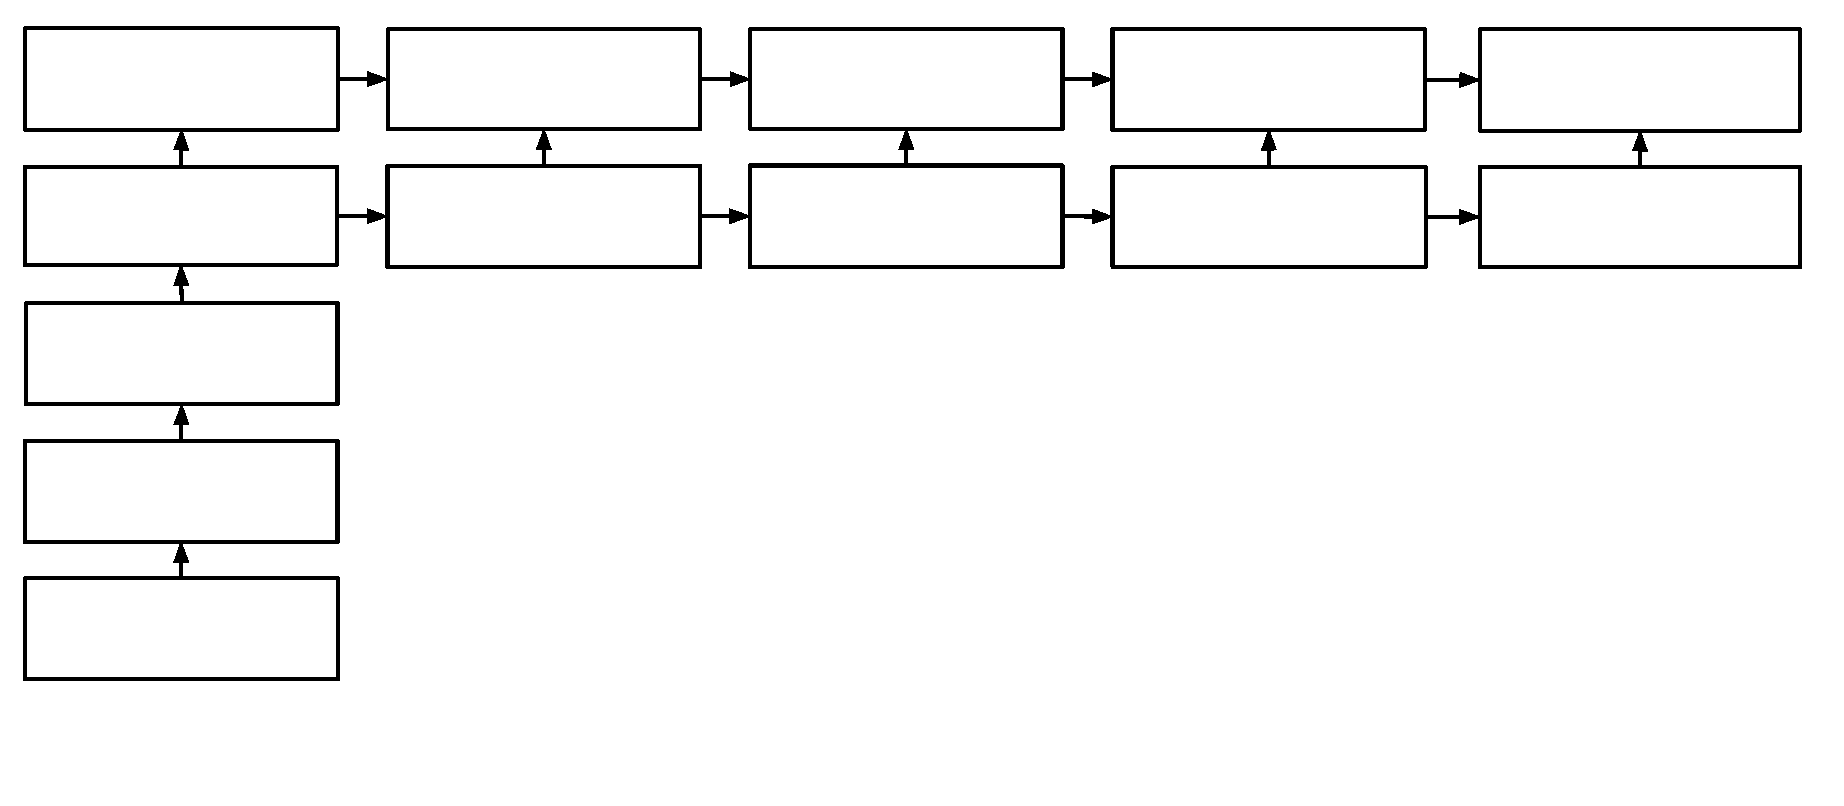
\includegraphics[width=\textwidth]{possible_pairs_of_states_of_parent_and_child_membrane}
    \caption{Possible pairs of states of parent and child membrane}
    \label{fig:possible_pairs_of_states_of_parent_and_child_membrane}
  \end{figure}

  \begin{figure}
    \def\svgwidth{\textwidth}
    \input{snapshot_of_all_membrane_states_while_simulating.pdf_tex}
    % 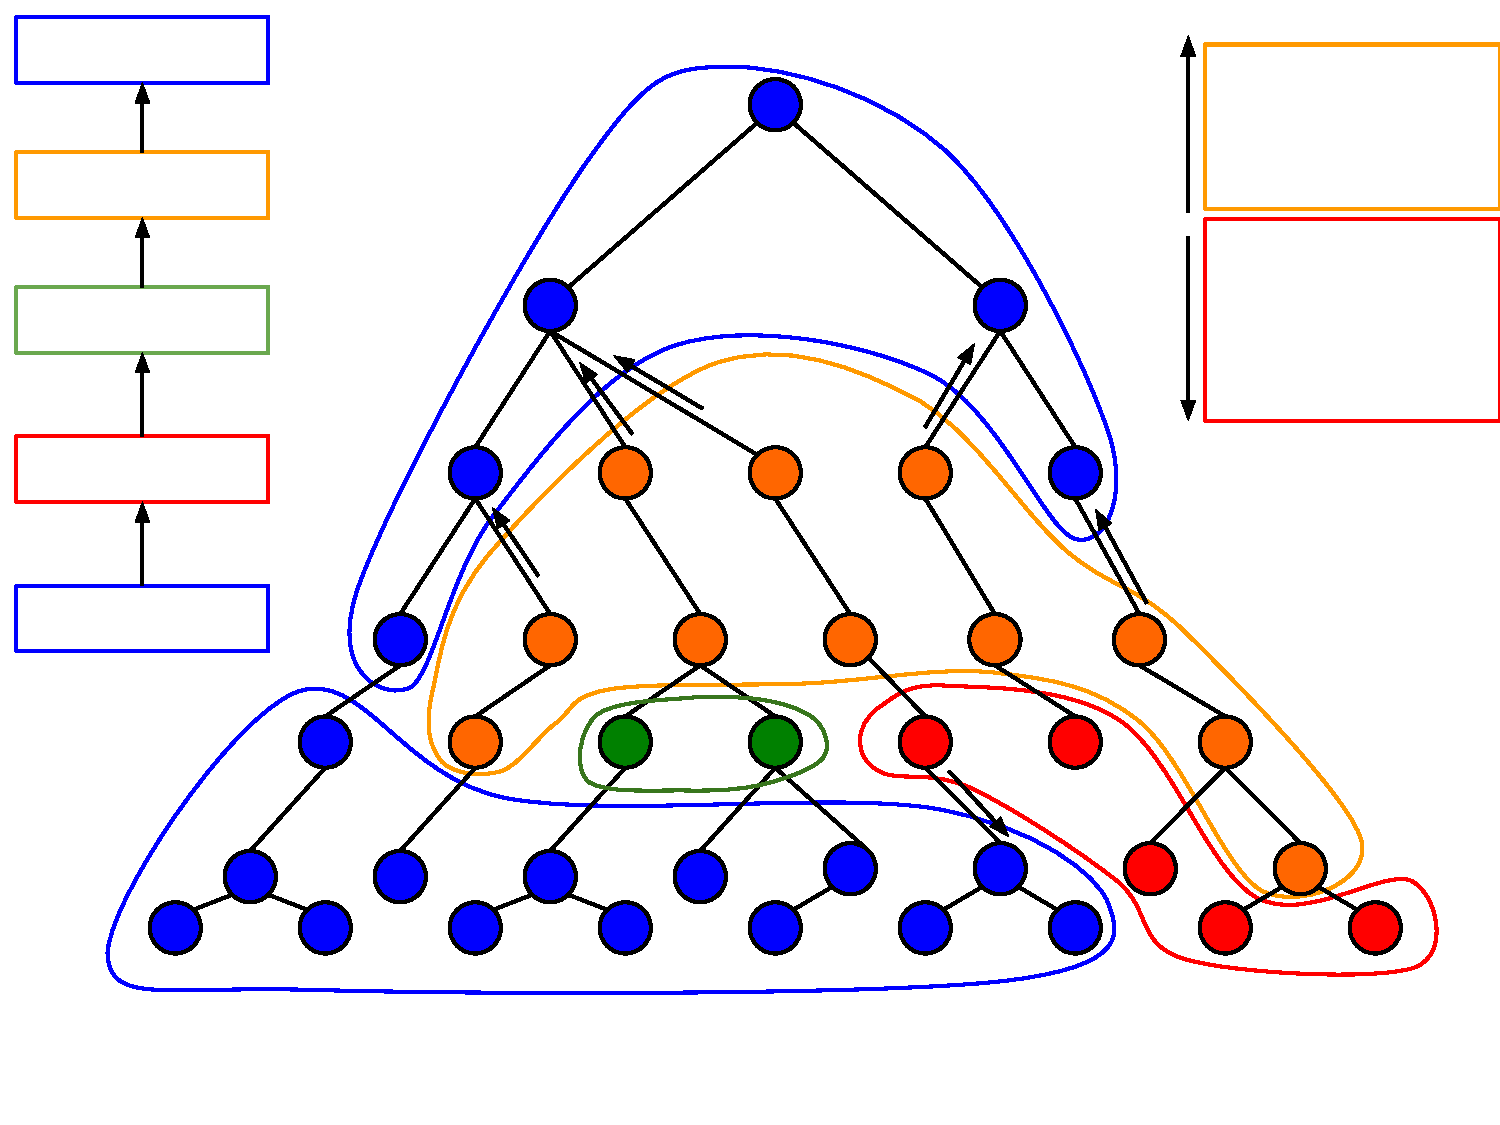
\includegraphics[width=\textwidth]{snapshot_of_all_membrane_states_while_simulating}
    \caption{Snapshot of all membrane states while simulating}
    \label{fig:snapshot_of_all_membrane_states_while_simulating}
  \end{figure}

  The pairs of possible phases of the parent and child membrane are shown in the figure \ref{fig:possible_pairs_of_states_of_parent_and_child_membrane} along with transitions between two consecutive global synchronizations - after the maximal parallel steps $i$ and $i+1$.

  In the figure \ref{fig:snapshot_of_all_membrane_states_while_simulating} the membrane structure is presented as a hierarchical structure. Every membrane is in one of four phases. It can be seen that the sending of the objects is performed in such phases that the receiving membrane is in either $RUN$ or $SYNCHRONIZE$ phase, so the received objects (marked $a^\prime$) does not interfere with rewriting.

  Another interesting idea can be seen in the figure \ref{fig:snapshot_of_all_membrane_states_while_simulating} that when a region is in the $SENDDOWN$ phase and objects are sent through the child membrane, the receiving region is in the $SYNCHRONIZE$ phase waiting for the $SYNCED$ signal, which will be sent to it when $SENDDOWN$ and $RESTORE$ phases finished.

  All membranes are nonempty during the simulation because at least the object representing the current phase is always present. By lemma~\ref{lemma:inhibitor_step} the rules with set of inhibitors can be simulated by single inhibitors.


\end{dokaz}




\subsection{Register machines} % (fold)
\label{sub:register_machines}
  We will use in our paper the power of Minsky's register machine \cite{Ionescu:jucs_10_5:on_p_systems_with}, that is why we recall here this notion. Such a machine runs a program consisting of numbered instructions of several simple types. Several variants of register machines with different number of registers and different instructions sets were shown to be computationally universal (see \cite{Ibarra:2005:SPS:2111772.2111880} for some original definitions and \cite{Khrisna03threeuniversality} for the definition used in this paper).

  \begin{definition}
  A {\bf $n$-register machine} is a tuple $M = (n,P,i,h)$, where:
  \begin{itemize}
    \item $n$ is the number of registers,
    \item $P$ is a set of labeled instructions of the form $j : (op(r),k,l)$, where $op(r)$ is an operation on register $r$ of $M$, and $j$, $k$, $l$ are labels from the set $Lab(M)$ (which numbers the instructions in a one-to-one manner),
    \item $i$ is the initial label, and
    \item $h$ is the final label.
  \end{itemize}
\end{definition}

The machine is capable of the following instructions:
\begin{itemize}
\item $(add(r),k,l)$ : Add one to the contents of register $r$ and proceed to instruction $k$ or to instruction $l$; in the deterministic variants usually considered in the literature we demand $k = l$.
\item $(sub(r),k,l)$ : If register $r$ is not empty, then subtract one from its contents and go to instruction $k$, otherwise proceed to instruction $l$.
\item $halt$ : This instruction stops the machine. This additional instruction can only be assigned to the final label $h$.
\end{itemize}

A deterministic $m$-register machine can analyze an input $(n_1,\dots,n_m)\in N_0^m$ in registers 1 to $m$, which is recognized if the register machine finally stops by the halt instruction with all its registers being empty (this last requirement is not necessary). If the machine does not halt, the analysis was not successful.
  
% subsection register_machines (end)

\subsection{Accepting vs generating} % (fold)
\label{sub:accepting_vs_generating}
  According to \cite{Barbuti:2010:MSW:1946067.1946081}, a P system can be used either as an acceptor or as a generator of a multiset language over $\Sigma$. In the first case, a multiset over $\Sigma$ is inserted in the skin membrane of the P system and the result of its computations says whether such a multiset belongs to the multiset language accepted by the P system or not. In the second case the P system has a fixed initial configuration and can give as results (possibly in a non-deterministic way) all the possible multisets belonging to a given multiset language.

% subsection accepting_vs_generating (end)

\subsection{Universality results for accepting case} % (fold)
\label{sub:universality_results_for_accepting_case}

% !TEX root = ../diz.tex
\begin{veta}
  Sequential P systems with cooperative rules and inhibitors can simulate register machines and thus equal $PsRE$.
\end{veta}


\begin{dokaz}
\label{proof:reg_by_inh}
  Suppose we have an $n$-register machine $M = (n,P,i,h)$. In our simulation we will have a membrane structure consisting of single membrane and the contents of register $j$ will be represented by the multiplicity of the object $a_j$.

  We will simulate the register machine by P system $(\Sigma, \mu, w, R)$, where:
  \begin{itemize}
    \item $\Sigma$ is an alphabet consisting of symbols that represent registers $a_1,\dots a_n$, instruction labels from the register machine $M$ and a halting symbol $\#$,
    \item $\mu$ is a membrane structure consisting of one single membrane,
    \item $w$ is initial contents of the membrane. It contains symbols for the input for the machine $a_i^{n_i}$ where $n_i$ is initial state of register with label $i$ and initial instruction label $e$.
    \item $R$ is a set of rules in the skin membrane.
  \end{itemize}
    
  For all instructions of type $(e : add(j), k, l)$ we will have rules:
  \begin{align*}
    e \rightarrow a_j|k\\
    e \rightarrow a_j|l.
  \end{align*}

  For all instructions of type $(e : sub(j), k, l)$ we will have rules:
  \begin{align*}
    e|a_j \rightarrow k\\
    e \rightarrow l|_{\neg a_j}.
  \end{align*}

  And finally halting rules:
  \begin{align*}
    h|a_j \rightarrow h|\#\text{~for all~}a\leq j\leq n,\\
    \# \rightarrow \#.
  \end{align*}

  For a configuration $(j, m_1, \dots, m_n)$ of the simulated register machine $M$ the skin membrane of the simulating P system contains a symbol $j$ and objects representing contents of registers $a_1^{m_1}, \dots, a_n^{m_n}$.

  When the halting instruction is reached, if there is an object present in the membrane, the hash symbol $\#$ is created and the rule $\# \rightarrow \#$ will be applicable forever as there is no rule to remove the symbol $\#$. If there is no object present, there is no rule to apply and computation will halt. It corresponds to the condition that all registers should be empty when halting. \qed
\end{dokaz}

% subsection universality_results_for_accepting_case (end)

\section{Trading maximal parallelism for vacuum}
\label{sec:vacuum}

In this section we will research how the vacuum object can help achieving universality.

\begin{veta}
  The sequential P system with Vacuum is universal.
\end{veta}

\begin{dokaz}
  We can simulate the variant of P system where the only cooperative rule is of type $a|a \rightarrow b$. According to \cite{Ibarra04dang} the variant, where the only cooperative rule is when both objects are the same, is universal. If there is no rule $a \rightarrow b$, we can rewrite $a$ to $a^{\prime}$ so we can mark all present symbols. $a^{\prime}$ symbols are kept in special membrane so the Vacuum can be created in main membrane and we can synchronize.
  
  But we won't do this madness again.
  
  Instead, we will try to prove universality by simulating the register machine. We need to detect when the current register is empty. If there was a symbol for every register as in the proof~\ref{proof:reg_by_inh}, the Vacuum would be created only if all registers are empty. But the $sub()$ instruction need to detect when one concrete register is empty.
  
  We will have a membrane for each register. That membrane will be contained in the skin membrane. The number of objects in membrane $i$ will correspond to the value of register $i$.
  
  The alphabet will consist of instruction labels and register counter $a$. The skin membrane will only have an instruction label. It is sent to corresponding membrane where the instruction is executed. Then, the following instruction is sent back to the skin membrane.
  
  We will have following rules in the skin membrane:
  
  \begin{itemize}
  \item $e \rightarrow e\downarrow_j$ for an instruction of type $e : add(j), f$ or $e : sub(j), f, z$ and
  \item $h \rightarrow h\downarrow$ for a halting instruction h.
  \end{itemize}
  
  And in non-skin membranes:
  
  \begin{itemize}
  \item $e \rightarrow a|f\uparrow$ instructions of type $e : add(j), f$,
  \item $e|a \rightarrow f\uparrow$ for instructions of type $e : sub(j), f, z$,
  \item $e|VACUUM \rightarrow z\uparrow$ for instructions of type $e : sub(j), f, z$, and
  \item $h|a \rightarrow h|a$
  \end{itemize}

  When halting, if there is an nonempty register, it will cycle forever with the last rule. However, if all registers are empty, the halting instruction label will stay in all membranes and the computation will halt.
  
\end{dokaz}

\section{Conclusion}
\label{sec:conclusion}
We have studied several variants of sequential P systems in order to obtain universality without using maximal parallelism.
A variant with rewriting rules that can use inhibitors was shown to be universal in both generating and accepting case. The generating model is able to simulate maximal parallel P system and the accepting model can simulate a register machine.

In addition, we have defined a new notion of vacuum, which is immediately created in the region that becomes empty. A new P system variant was introduced, which allowed the vacuum to be used on the left side of P system rewriting rules. The accepting case of this variant was shown to be universal by direct implementation of a register machine.

A lot of other variants deserve to be combined with the vacuum, so we suggest to research them more thoroughly(non-cooperative rules, rules with priorities, decaying objects, deterministic steps, \dots).

\bibliography{inh}
\end{document}
